
\subsection{Datamodeller}

\begin{figure*}[t]
\centering
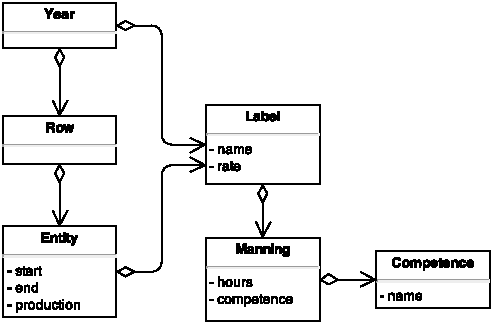
\includegraphics[width=0.6\textwidth]{model.pdf}
\caption{UML-diagram för de relevanta delarna av systemet}
\label{fig:model}
\end{figure*}

Ett förenklat UML-diagram för de relevanta delarna av systemet visas i
Figur \ref{fig:model}. Tanken är att den befintliga datamodellen i
framtiden kan utökas med klassen \emph{Manning}. Ett sådant objekt
representerar en bemanning som krävs för en viss typ av aktivitet, t.ex.
en viss typ av personal som ska jobba ett visst antal timmar. I
framtiden kan varje sådan bemanning även kräva en eller flera
kompetenser.\\

Uppdragsgivaren vill undvika en onödigt komplicerad datastruktur i den
händelse att systemet inte kommer att utökas med mer komplexa krav på
modellen. Därför kommer till en början ett attribut på klassen
\emph{Label} att användas för att beskriva antalet bemannade timmar,
istället för att utöka datamodellerna med en ny klass. Skapandet av en
separat \emph{Manning}-klass skulle i så fall kräva en mindre
datamigrering.\\

Om det finns ett behov av att följa upp faktisk bemanning, kan detta
lösas med ett nytt attribut för antal bemannade timmar på klassen
\emph{Entity}.


\subsection{Användargränssnitt}

Vi tror att det smidigaste alternativet är att kunna byta mellan olika
lägen i användargränssnitten, beroende på om man vill visa planerad
bemanning eller planerad produktion. En svårighet är att representera
detta på ett bra sätt för användaren, då till synes likadana siffror
då får radikalt olika betydelse beroende på i vilket läge man befinner
sig. Därav kommer framtagningen av gränssnittet ske iterativt, där
olika versioner kan utvärderas i samarbete med systemets användare.\\

En central del är den totala summan av antalet bemannade timmar. Detta
tillhandahålls i användargränssnittet som en möjlighet att se
summeringar för timmarna. Det vore troligen lämpligt att kunna summera
dessa såväl totalt och per veckodag som per aktivitet.\\
